\documentclass{beamer}

\mode<presentation> {
%  \usetheme{Warsaw}
	\usetheme{metropolis} 
}

\setbeamertemplate{footline}[frame number]
\addtocounter{framenumber}{-1}

%\usepackage{ucs}
\usepackage[utf8]{inputenc}
\usepackage[czech]{babel}
%\usepackage{palatino}
\usepackage{graphicx}
\usepackage{listings}
\usepackage{fontawesome}

\title[BitLocker disk encryption on Linux]{BitLocker disk encryption on Linux}
\author{Vojtěch Trefný\\ \small \texttt{mail@vojtechtrefny.cz}\\}
\date{DevConf CZ, 25. 1. 2020\\}
 \institute{\faTwitter\, \href{https://twitter.com/vojtechtrefny}{twitter.com/vojtechtrefny} \\ \faGithub\, \href{https://github.com/vojtechtrefny}{github.com/vojtechtrefny} \\ \faGitlab\ \href{https://gitlab.com/vtrefny}{gitlab.com/vtrefny}}

\begin{document}

{\setbeamertemplate{footline}{} 
\begin{frame}
\titlepage
\end{frame}
}

%%%%%%%%%%%%%%%%%%%%%%%%%%%%%%%%%%%%%%%%%%%%%%%%%%%%%%%%%%%%%%%%%%

\section{BitLocker}

\begin{frame}
	\frametitle{BitLocker}

	\begin{block}{}
		\begin{itemize}
			\item Native full disk encryption for Microsoft Windows.
			\item First introduced in 2006 in Windows Vista.\footnotemark
			\begin{itemize}
				\item A new version of on-disk metadata was introduced in Windows~7.
				\item New algorithms for the data encryption introduced in Windows~8 (AES-CBC) and Windows~10 (AES-XTS).
			\end{itemize}
			\item Supports encryption of both system drive and removable devices (BitLocker ToGo).
			\item The on-disk metadata format is not open but there is enough public information and we have existing opensource implementations for Linux\footnotemark.
		\end{itemize}
	\end{block}
\footnotetext[1]{\tiny FERGUSON, Niels. AES-CBC + Elephant diffuser: A Disk Encryption Algorithm for Windows Vista.}
\footnotetext[2]{\tiny Detailed description of the metadata by Joachim Metz is available in the \href{https://github.com/libyal/libbde/blob/master/documentation/BitLocker\%20Drive\%20Encryption\%20(BDE)\%20format.asciidoc}{\underline{libbde documentation}}.}
\end{frame}

\begin{frame}
	\frametitle{Why BitLocker?}
	
	\begin{block}{}
		\begin{itemize}
			\item There currently isn’t a technology for full disk encryption that would work seamlessly,
without installing additional tools, in Microsoft Windows, GNU/Linux or both.
			\item Existing tools for Linux are not very user-friendly and use FUSE and custom implementations of cryptographic functions.
			\item Ideally, BitLocker devices would be automatically recognized and presented to the user in the same way native encrypted devices are.
		\end{itemize}
	\end{block}
\end{frame}

\begin{frame}
	\frametitle{BitLocker device structure}

	\begin{block}{}
		\begin{itemize}
			\item \textbf{Header} -- format identification and FVE metadata offsets.
			\item \textbf{FVE metadata} -- BitLocker configuration and keys.
			\item \textbf{NTFS header} -- encrypted header for the open device.
			\item \textbf{Encrypted data}.
		\end{itemize}
	\end{block}
	
	\begin{figure}[ht!]
	\begin{center}
  	  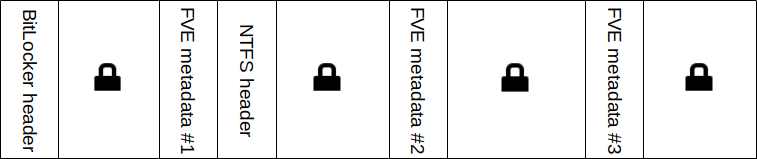
\includegraphics[width=11cm]{img/bitlocker-schema.png}
	\end{center}
	\end{figure}

\end{frame}

\begin{frame}
	\frametitle{Keys}

	\begin{block}{}
		\begin{itemize}
			\item BitLocker metadata contain two types of keys:
				\begin{itemize}
					\item \textbf{FVEK} is a 128 or 256 bit key used for data encryption and
					\item \textbf{VMK} is used to decrypt FVEK. Multiple encrypted copies of the VMK are stored in the metadata with different types of protectors.
				\end{itemize}
		\end{itemize}
	\end{block}
	\begin{figure}[ht!]
	\begin{center}
  	  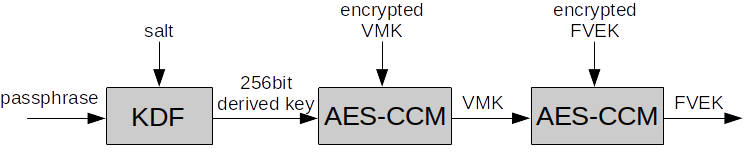
\includegraphics[width=11cm]{img/keys.png}
	\end{center}
	\end{figure}

\end{frame}

%%%%%%%%%%%%%%%%%%%%%%%%%%%%%%%%%%%%%%%%%%%%%%%%%%%%%%%%%%%%%%%%%%

\section{Disk encryption on Linux \\ \small Device Mapper and LUKS}

\begin{frame}
	\frametitle{Device Mapper}

	\begin{block}{Device Mapper}
		\begin{itemize}
			\item Kernel module for creating ``mapped'' virtual block devices.
			\item Can be used to ``partition'' disks to smaller block devices or to concatenate multiple disks to one volume.
			\item Multiple \emph{targets} provide additional features that include encryption, caching, mirroring etc.
		\end{itemize}
	\end{block}
	
	\begin{block}{dm-crypt}
		\begin{itemize}
			\item Crypt target provides transparent disk encryption.
			\item Data written to a dm-crypt device are encrypted with provided key and cipher specification before writing them to the underlying block device.
		\end{itemize}
	\end{block}

\end{frame}

\begin{frame}[fragile]
	\frametitle{LUKS}
	\begin{block}{Using dm-crypt directly is not very user-friendly}
	\begin{lstlisting}[frame=none, basicstyle=\ttfamily\small, columns=fullflexible, keepspaces=true]
# dmsetup create x --table "0 204800 crypt aes-xts-plain64 
9d3...d5c 0 /dev/sdb1 0 0"\end{lstlisting}
	\end{block}

	\begin{block}{LUKS}
		\begin{itemize}
			\item Linux Unified Key Setup
			\item Defines a standardized format for storing metadata and key materials.
			\item Allows simple and user-friendly way of creating and managing of encrypted devices.
		\end{itemize}
	\end{block}

	\begin{lstlisting}[frame=none, basicstyle=\ttfamily\small, columns=fullflexible, keepspaces=true]
# cryptsetup luksOpen /dev/sdb1 x
Enter passphrase for /dev/sdb1: ***\end{lstlisting}

\end{frame}

\begin{frame}
	\frametitle{BitLocker vs. LUKS}
	\begin{figure}[ht!]
	\begin{center}
  	  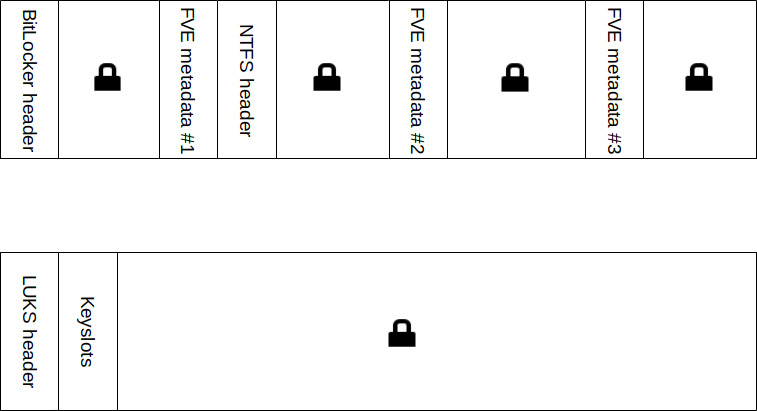
\includegraphics[width=11cm]{img/luks-bitlocker.png}
	\end{center}
	\end{figure}
	
\end{frame}

\section{BitLocker on Linux}

\begin{frame}
	\frametitle{BitLocker and Device Mapper}

	\begin{block}{Device Mapper needs to know:}
		\begin{itemize}
			\item cipher (AES-XTS for Windows 10),
			\item initialization vector (sector number),
			\item key and
			\item location (offset) of the encrypted data.
		\end{itemize}
	\end{block}
\vspace{-0.25cm}
\begin{figure}[ht!]
	\begin{center}
  	  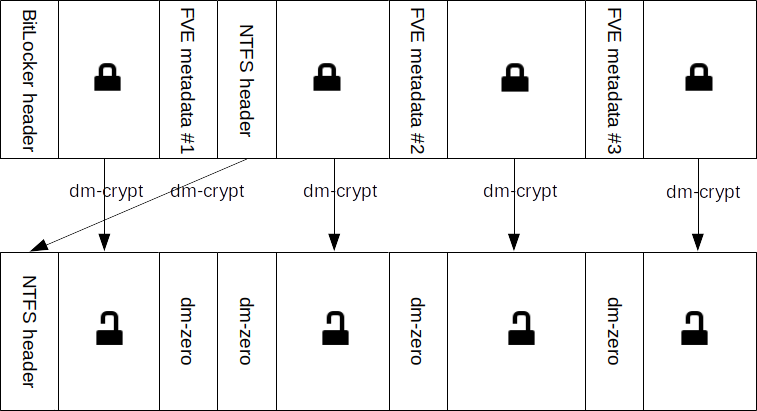
\includegraphics[width=9cm]{img/bitlocker-dm-schema.png}
	\end{center}
	\end{figure}

\end{frame}

\begin{frame}[fragile]
\frametitle{BitLocker and Device Mapper}
\begin{block}{Using Device Mapper directly is not very user-friendly}
	\begin{lstlisting}[frame=none, basicstyle=\ttfamily\small, columns=fullflexible, keepspaces=true]
# dmsetup table --showkeys
x: 0 16 crypt aes-xts-plain64 cc4...d66 68904 7:0 68904
x: 16 68760 crypt aes-xts-plain64 cc4...d66 16 7:0 16
x: 68776 128 zero 
x: 68904 16 zero 
x: 68920 21424 crypt aes-xts-plain64 cc4...d66 68920 7:0 68920
x: 90344 128 zero 
x: 90472 22632 crypt aes-xts-plain64 cc4...d66 90472 7:0 90472
x: 113104 128 zero 
x: 113232 91568 crypt aes-xts-plain64 cc4...d66 113232 7:0 \
	113232
	\end{lstlisting}
\end{block}
\end{frame}

\begin{frame}[fragile]
	\frametitle{BitLocker in cryptsetup}

	\begin{block}{}
		\begin{itemize}
			\item Support for BITLK (BitLocker compatible) devices was added in cryptsetup 2.3.0\footnotemark.
			\item Cryptsetup can now parse BitLocker metadata, extract and decrypt (password protected) keys and construct the multi segment device mapper device.
		\end{itemize}
	\end{block}

\vspace{0.25cm}
	
\begin{lstlisting}[frame=none, basicstyle=\ttfamily\small, columns=fullflexible, keepspaces=true]
# cryptsetup bitlkOpen /dev/sdb2 x
Enter passphrase for /dev/sdb2: ***
\end{lstlisting}

\footnotetext[5]{\tiny cryptsetup 2.3.0-rc0 was released on Jan 12, 2020.}
\end{frame}

\begin{frame}[fragile]
	\frametitle{BitLocker in cryptsetup}

\begin{lstlisting}[frame=none, basicstyle=\ttfamily\small, columns=fullflexible, keepspaces=true]
# cryptsetup bitlkDump /dev/sdb2
Info for BITLK device /dev/sdb2.
Version:        2
GUID:           8f595209-f5b9-49a0-85d4-cb8f80258c27
Created:        Thu Jul  4 09:01:55 2019
Description:    DESKTOP-NPM7RCA H: 7/4/2019
Cipher name:    aes
Cipher mode:    xts-plain64
Cipher key:     128 bits

Keyslots:
 0: VMK
        GUID:           3e55195c-8811-4d9b-97b4-2b9e5f8f5384
        Protection:     VMK protected with passphrase
        Salt:           8d7637cc5d885d5ff4f748dbc8440d2e
        Key data size:  44 [bytes]
...
\end{lstlisting}

\end{frame}

\begin{frame}
	\frametitle{Supported features}
	
	\begin{block}{Protectors}
		\begin{itemize}
			\item \emph{Supported:} passphrase, recovery passphrase
			\item \emph{Unsupported:} TPM, smart cards, startup key...
		\end{itemize}
	\end{block}

	\begin{block}{Encryption}
		\begin{itemize}
			\item \emph{AES-XTS} (Windows 10): supported in all versions
			\item \emph{AES-CBC} (Windows 7-10): Linux 5.3
			\item \emph{AES-CBC + Elephant diffuser} (Windows Vista): Linux 5.6
		\end{itemize}
	\end{block}

	\begin{block}{Metadata}
		\begin{itemize}
			\item Only version 2 (Windows 7+) is supported.
		\end{itemize}
	\end{block}
\end{frame}

\begin{frame}
	\frametitle{BitLocker in UDisks}
	\begin{itemize}
		\item UDisks is a daemon for accessing and manipulating with disks and storage devices.
		\item It's used to mount and open removable devices in most graphical environments.
		\item BitLocker devices are identified by udev (using libblkid\footnotemark).
		\item UDisks provides the \texttt{Encrypted} DBus interface for BitLocker devices and \texttt{Unlock} and \texttt{Lock} functions for (un)locking these devices.
		\item No further changes are needed in the GUI tools and daemons like GVfs to support BitLocker.
		\item Support for BitLocker will be available in UDisks 2.9.0.
	\end{itemize}

\footnotetext[6]{\tiny Detection of BitLocker devices was added in util-linux v2.33.}
\end{frame}

\begin{frame}[fragile]
	\frametitle{BitLocker in UDisks}

	\begin{lstlisting}[frame=none, escapechar=$, basicstyle=\ttfamily\small, columns=fullflexible, keepspaces=true]
/org/freedesktop/UDisks2/block_devices/sdb2:
  org.freedesktop.UDisks2.Block:
...
    Id:
    IdLabel:
    $\textcolor{blue}{IdType:}$                     $\textcolor{blue}{BitLocker}$
    $\textcolor{red}{IdUUID:}$                     $\textcolor{red}{1f8bf933-8323-4c97-...}$
    $\textcolor{blue}{IdUsage:}$                    $\textcolor{blue}{crypto}$
  $\textcolor{red}{org.freedesktop.UDisks2.Encrypted:}$
    ChildConfiguration:         []
    CleartextDevice:            '/'
    $\textcolor{red}{HintEncryptionType:}$          $\textcolor{red}{BitLocker}$
\end{lstlisting}

\end{frame}

%%%%%%%%%%%%%%%%%%%%%%%%%%%%%%%%%%%%%%%%%%%%%%%%%%%%%%%%%%%%%%%%%%

\section{Summary}

\begin{frame}
	\frametitle{Questions}

	\begin{center}
	Thank you for your attention.
	\end{center}

\vspace{0.5cm}

	\begin{center}
	Please test BITLK support in cryptsetup and report all bugs at \href{https://gitlab.com/cryptsetup/cryptsetup/issues}{gitlab.com/cryptsetup/cryptsetup/issues}
	\end{center}
\end{frame}

\end{document}

